\chapter{Background}
\label{ch:background}

This work examines the relationship between system and application performance in the context of systems comprised of CPUs and NVIDIA GPUs.
To that end, this section describes
\begin{itemize}
\item How NVIDIA GPUs fit into the computing system architecture (Section~\ref{sec:gpu-sys-arch}).
\item Common system interconnects used to couple GPUs to each other and the rest of the system (Section~\ref{sec:interconnects}).
\item Communication-related components of CUDA, the NVIDIA GPU programming system (Section~\ref{sec:cuda}).
\item The relationship between CUDA's abstractions and the underlying system hardware (Section~\ref{sec:sys-abstraction}).
\item The Linux and CUDA components used by the application profiler (Section~\ref{sec:profiling}).
\item The heterogeneous systems used as case studies in this work (Section~\ref{sec:system-descriptions}).
\end{itemize}

\section{GPUs and System Architecture}
\label{sec:gpu-sys-arch}

Most GPUs used in high-performance computing are fully-discrete accelerators.
From the software side, they demand explicit management through esoteric programming systems.
The CPU typically acts as a manager,  and ``offloads'' specialized compute tasks to the GPU.
From the hardware perspective, GPUs are separated from the CPU and system storage by a local interconnect link.
The GPU has its own local memory, which must be populated with data for the GPU to operate on.
Finally, though not covered in this work, the GPU compute cores have dramatically different performance characteristics than CPU cores, and require specialized programming styles.


\begin{figure}[ht]
    \centering
    \begin{subfigure}[b]{0.2\textwidth}
        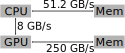
\includegraphics[width=\textwidth]{figures/generated/x86-kepler-bw.pdf}
        \caption{AMD Opteron 6200 / PCIe 2.0 / K20X }
        \label{fig:x86-kepler-bw}
    \end{subfigure}
	~
	\begin{subfigure}[b]{0.2\textwidth}
        \includegraphics[width=\textwidth]{figures/generated/x86-pascal-bw.pdf}
        \caption{Intel Xeon Platinum 8180M / PCIe 3.0 / Pascal P100}
        \label{fig:x86-pascal-bw}
    \end{subfigure}
    ~
    \begin{subfigure}[b]{0.2\textwidth}
        \includegraphics[width=\textwidth]{figures/generated/p8-pascal-bw.pdf}
        \caption{Power8 / NVLink / Pascal}
        \label{fig:p8-pascal-bw}
    \end{subfigure}
    ~
    \begin{subfigure}[b]{0.2\textwidth}
        \includegraphics[width=\textwidth]{figures/generated/p9-volta-bw.pdf}
        \caption{Power9 / NVLink / Volta}
        \label{fig:p9-pascal-bw}
    \end{subfigure}
    \caption[\todo{short}]{Relative interconnect bandwidths of some hypothetical systems. \cite{amd2012opteron6200} \cite{stuechli2013power8}}.
    \label{fig:gpu-sys-arch}
\end{figure}

Figure~\ref{fig:gpu-sys-arch} shows some example interconnect bandwidth numbers for some hypothetical systems.
In all cases, the bandwidth between the CPU or GPU and their respective memories is much higher than the bandwidth between the CPU and GPU.
Figure~\ref{fig:x86-kepler-bw} is representative of a node of a supercomputer designed in 2012.
Figure~\ref{fig:x86-pascal-bw} represents a similar system, with components updated to 2017.
Figure~\ref{fig:p8-pascal-bw} is a c.2014 system with an IBM Power8 CPU and NVLink.
Figure~ref{fig:p9-volta-bw} represents next-generation link bandwidths coming online in the Summit\todo{cite} and Sierra\todo{cite} supercomputers.

\section{Interconnects}
\label{sec:interconnects}

Modern systems with discrete GPUs typically feature one of two kinds of common accelerator interconnects.
These interconnects may couple the GPUs to the CPUs and/or other GPUs.
Table~\ref{tab:interconnect-overview} summarizes the theoretical bandwidth of common interconnect configurations.
Figure~\ref{fig:interconnect-cartoon} shows example PCIe and NVLink topologies.
Section~\ref{sec:cuda-peer} describes how these topologies affect parts of the CUDA peer-communication API.

\begin{table}[h]
	\centering
	\caption[Interconnect Performance Summary]{
		Theoretical performance for common interconnect configurations.
		Most PCIe 3.0-attached GPUs use 16 lanes, or PCIe x16.
		The IBM ``Minsky'' system, described in Section~\ref{}, uses two NVLink 1.0 lanes to connect pairs of devices, with each lane operating at 20 GB/s~\cite{nvidia2016p100}.
		The IBM Power9 / Volta system, described in Section~\ref{}, uses three NVLink 2.0 lanes to connect pairs of devices, with each lane operating at 25 GB/s~\cite{nvidia2017v100}.
	}
	\label{tab:interconnect-overview}
	\begin{tabular}{|c|c|c|c|}
		\hline
		\textbf{Interconnect} & \textbf{Bandwidth}  & \textbf{Year} & \textbf{Architecture}\\ \hline
		\textbf{PCIe 3.0}          & 12.8 GB/s (16 lanes) & 2010 & Tree   \\ \hline
		\textbf{NVLink 1.0 / NVHS} &   40 GB/s (2 lanes)  & 2016 & Point-to-Point \\ \hline
		\textbf{NVLink 2.0 / NVHS} &   75 GB/s (3 lanes)  & 2017 & Point-to-Point \\ \hline
	\end{tabular}
\end{table}

\begin{figure}[ht]
    \centering
	\begin{subfigure}[b]{0.4\textwidth}
		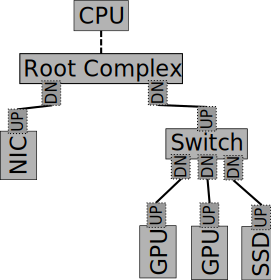
\includegraphics[width=\textwidth]{figures/generated/pcie-example.pdf}
		\caption[]{}
		\label{fig:pcie-cartoon}
    \end{subfigure}
    ~
    \begin{subfigure}[b]{0.4\textwidth}
		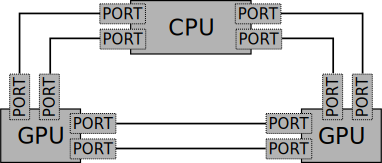
\includegraphics[width=\textwidth]{figures/generated/nvlink-example.pdf}
		\caption[]{}
		\label{fig:pcie-cartoon}
    \end{subfigure}
    \caption[Example PCIe and NVLink interconnect topologies]{
		(a): an example PCIe topology, showing the root complex at the root of the tree, with endpoints and switches connected by links.
		(b): an example NVLink topology, with each device supporting four NVLinks, and using two to connect to each of its neighbor devices.
		In both examples, a second CPU socket has access to the topopolgy, but must first have its communication pass through the CPU socket assocated with the interconnects.
	}
    \label{fig:interconnect-cartoon}
\end{figure}

\subsection{PCIe}

Peripheral Component Interconnect Express (PCIe) is an expansion bus standard~\cite{pcie10a}.
PCIe components form a tree, rooted at the \textit{root complex}.
PCIe devices such as GPUs or SSDs are \textit{endpoints}, with a single upstream port and no downstream ports.
Data is sent point-to-point between participating endpoints and/or the root complex via unique PCIe addresses.
The topology also may include \textit{switches}, components with a single upstream port and multiple downstream ports.
Switches do not receive data packes, and are only used to extend the topology.
Components are connected by PCIe \textit{links}, each of which consists of one to 32 lanes.
The total bandwidth of the link depends on the PCIe revision and the number of lanes.
Figure~\ref{fig:pcie-cartoon} shows an example topology.




\subsection{NVLink}

NVLink is a communication protocol developed by NVIDIA.
Current NVLink implementations use a proprietary High-Speed Signaling interconnect called NVHS \cite{harris2016insidepascal}.
Like PCIe, each NVLink connects two devices.
Unlike PCIe, there is no concept of upstream or downstream ports, and devices may have multiple ports.
Multiple links may connect devices, in which case the links are bonded and both contribute to the available bandwidth between devices.
Figure~\ref{fig:nvlink-cartoon} shows an example topology.




%
%
%
\section{Programming Systems}
\subsection{CUDA}
\label{sec:cuda}


NVIDIA's CUDA (Compute Unified Device Architecture) is a programming system for enabling general-purpose computation on NVIDIA GPUs (graphics processing units).
CUDA is a set of C extensions and libraries for interfacing with GPUs.
NVIDIA provides a compiler, \texttt{nvcc} for generating CUDA-enabled binaries.

CUDA provides a set of runtime and driver APIs for the developer to manage the allocation and movement of data between the host and device memory.
From its inception, CUDA provided comprehensive APIs for developers to mitigate application performance shortfalls stemming from the relatively limited performance of host-device communication links.
As the capabilities of GPUs and host systems have improved, CUDA has provided simpler, higher-level APIs that require less programmer effort.
This section describes CUDA memory-management capabilities and the historical context of their introduction.

The CUDA API has an associated version number that defines which CUDA actions are made available by that API.
CUDA-capable hardware advertises a specific compute capability (CC) that defines what CUDA actions are supported by that GPU.
Although the CUDA API may expose particular capability, the GPU may need a sufficiently high CC to take advantage of it.
This section references both these version systems when discussing CUDA features.

\subsection{CUDA Memory}

Prior to the introduction of Unified Virtual Addressing (see Section~\ref{sec:uva}), the CUDA memory space was composed of multiple address spaces: one for the host, and one for each GPU~\cite{schroeder2011peer}.
Data was explicitly allocated in and moved between those address spaces through the basic CUDA memory management runtime calls described in Table~\ref{tab:cuda-basic-apis}.
Standard C/C++ memory allocation techniques (\texttt{malloc}/\texttt{new}, \texttt{free}/\texttt{new}) are used for managing memory on the host.

\begin{table}[h]
	\centering
	\caption[Basic CUDA Memory-management APIs]{\todo{long caption}}
	\label{tab:cuda-basic-apis}
	\begin{tabular}{|c|c|}
		\hline
		\textbf{API}             & \textbf{Description}                        \\ \hline
		\texttt{cudaSetDevice()} & Associate a device with the host thread.    \\ \hline
		\texttt{cudaMalloc()}    & Allocate memory on the device.              \\ \hline
		\texttt{cudaFree()}      & Free memory on the device.                  \\ \hline
		\texttt{cudaMemcpy()}    & Copy data between to,from,and between GPUs. \\ \hline
		\texttt{cudaMemcpyPeer}  & Copy data between GPUs without CPU involved. \\ \hline 
	\end{tabular}
\end{table}

\texttt{cudaSetDevice} sets which device subsequent calls from the host thread will affect.
\texttt{cudaMalloc} is used to allocate memory that may be used in CUDA kernels.
\texttt{cudaMemcpy} is used to move data between the host and device, or between devices.
Since each device has a separate address space, the programmer explicitly instructs \texttt{cudaMemcpy} how to move data with \texttt{cudaMemcpyHostToDevice}, \texttt{cudaMemcpyDeviceToHost}, or \texttt{cudaMemcpyDeviceToDevice}.
\texttt{cudaMemcpyPeer} initiates a DMA copy from one GPU to another, without involving the host.

This API definition imposes the following basic structure on all CUDA programs, which remains essentially unchanged as of the writing of this document.
\begin{enumerate}
	\item allocate memory on the host with \texttt{new}/\texttt{malloc}.
	\item initialize memory on the host
	\item allocate memory on the device with \texttt{cudaMalloc}
	\item copy initialized data from the host to the device with \texttt{cudaMemcpy(..., cudaMemcpyHostToDevice)}
	\item launch CUDA kernels
	\item copy results back to the host with \texttt{cudaMemcpy(..., cudaMemcpyDeviceToHost)}
	\item free CUDA allocations with \texttt{cudaFree}
\end{enumerate}

Unified virtual addressing (Section~\ref{sec:uva}) and unified memory (Section ~\ref{sec:um}) allow the programmer to make some of these steps implicit.



\subsubsection{Page-Locked Memory}

The GPU uses direct memory access (DMA) to copy data to and from the host.
When \texttt{cudaMemcpy} is invoked, the CPU instructs the GPU to copy a region of host memory to the device memory (or vis-versa), without the CPU being involved.
The host must guarantee that the memory to be accessed by the GPU will not be paged-out during the copy.
First, \texttt{cudaMemcpy} copies the data from the application address space to a piece of page-locked memory in the system memory managed by the CUDA driver, and then \texttt{cudaMemcpy} instructs the GPU to initiate the DMA from that page-locked region to the GPU memory.

The CUDA runtime functions in Table~\ref{tab:cuda-pinned-apis} are the core functions CUDA provides to make page-locked memory regions directly visible to the application.
When the application uses these APIs, the first copy from pageable host memory to page-locked host memory can be elided.
Section \ref{sec:todo} demonstrates the performance improvement from skipping this first copy.
Overuse of page-locked memory on the host will degrade overall application performance or even impact system stability if the host system is not able to page as needed.

\begin{table}[h]
	\centering
	\caption[CUDA Pinned Memory-Management APIs]{\todo{long caption}}
	\label{tab:cuda-pinned-apis}
	\begin{tabular}{|c|c|c|}
		\hline
		\textbf{API}                & \textbf{Description}                    & \textbf{Introduced} \\ \hline
		\texttt{cudaMallocHost()}   & allocate page-locked memory on the host & 1.0~\cite{nvidia2007cuda10} \\ \hline
		\texttt{cudaFreeHost()}     & free page-locked memory on the host     & 1.0~\cite{nvidia2007cuda10} \\ \hline
		\texttt{cudaHostAlloc()}    & cudaMallocHost with additional options  & 3.0~\cite{nvidia2010cuda30} \\ \hline
		\texttt{cudaHostRegister()} & Page-lock a range of host memory        & 4.0~\cite{nvidia2011cudac40} \\ \hline
	\end{tabular}
\end{table}

\texttt{cudaHostAlloc} allows even more options, including the \texttt{cudaHostAllocPortable}, \texttt{cudaHostAllocMapped}, and \texttt{cudaHostAllocWriteCombined} flags.

%3.2.4.2
\texttt{cudaHostAllocWriteCombined} causes a pinned allocation to be write-combined.
Writes to write-combined memory may be delayed and combined in a buffer to reduce the number of memory accesses.
Additionally, the host may not cache this data in L1 or L2 cache, freeing up those resources for other applications. 
\todo{why only L1 and L2?}
Furthermore, coherency is not enforced, so data is not snooped on the PCIe bus, which can increase bandwidth by up to 40\% (\cite{nvidia2010cuda30}, 3.2.5.2).
This type of allocation makes sense for data that is not frequently read by the CPU, for example, data written once by the CPU before being sent to a GPU.

%3.2.4.3 
\texttt{cudaHostAllocMapped} introduces the ability to map the host allocation (in the host address space) into the device's address space.
By using \texttt{cudaHostGetDevicePointer}, the corresponding pointer in the device address space may be obtained and directly used by CUDA kernels.
In this case, the programmer does not need to explicitly allocate memory or copy data to the device, nor does the programmer need to use streams to overlap computation with communication.

\texttt{cudaHostAllocPortable} allows all CUDA contexts to treat the memory as pinned, not just the context that performed the allocation.
This became the default with the introduction of unified virtual addressing. \todo{why not have this from the start? Is there a performance cost? 3.2.5.1 of CUDA 3.0}.

\subsubsection{Unified Virtual Addressing}
\label{sec:uva}

Unified Virtual Addressing was introduced with compute capability 2.0 GPUs and CUDA 4.0 on 64-bit systems.
The host memory and the memory of each GPU are mapped into disjoint subsections of a single unified address space.

This enhancement simplifies several of the already-introduced CUDA memory management commands~(\cite{nvidia2011cudac40}, 3.2.7).
The \texttt{cudaMemcpyDefault} flag for \texttt{cudaMemcpy} instructs the CUDA system to automatically determine how to move data.
By examining the address of the pointers passed to \texttt{cudaMemcpy}, CUDA determines where which device the memory resides on and moves it accordingly.
This simplifies the programmer's use of \texttt{cudaMemcpy}, as \texttt{cudaMemcpyDefault} may be used everywhere.
There is also no need to call \texttt{cudaHostGetDevicePointer} for mapped allocations.
Furthermore, all mapped allocations are autmatically portable between GPUs, not restricted to the GPU that was active at the time of the allocation.
\texttt{cudaMemcpyPeer} is no longer needed for device-to-device memory copies; \texttt{cudaMemcpy} may be used instead.

\subsubsection{Peer Access and UVA}
\label{sec:cuda-peer}

Peer access was introduced with CUDA 4.0.
\texttt{cudaDeviceEnablePeerAccess()} allows CC 2.0+ devices to address memory in another device's address space~(\cite{nvidia2011cudac40}, 3.2.6.4).
For example, if GPU1 loads through a pointer to data on GPU0, the data will be directly fetched from GPU0 memory, at the cost of one PCIe transasction and one globably memory load, and be cached in the L2 of GPU0.
Direct peer access requires compute capability 2.0, CUDA 4.0,Fermi+, and 64-bit system~\cite{schroeder2011peer}.
The availablility of peer access may rely on a combination of interconnect topology and system hardware.

\begin{table}[h]
	\centering
	\caption[\todo{short}]{\todo{long}}
	\label{tab:cuda-peer-topology}
	\begin{tabular}{|c|c|c|}
		\hline
		\textbf{System} & \textbf{Configuration} & \textbf{Peer Access} \\ \hline
		\todo{system} & shared switch  & Yes \\ \hline
		\todo{system} & different switches  & No \\ \hline
		IBM ``Minsky'' & direct NVLink connection  & Yes \\ \hline
		IBM ``Minsky'' & no direct NVLink connection  & No \\ \hline
		IBM P9 / Volta & direct NVLink connection  & Yes \\ \hline
		IBM P9 / Volta & no direct NVLink connection  & Yes \\ \hline

	\end{tabular}
\end{table}



\subsubsection{Unified Memory with CC 3.0+ (Kepler+)}

\begin{itemize}
	\item cudaMallocManaged (cudaMemAttachHost, cudaMemAttachGlobal)
\end{itemize}


\texttt{cudaDeviceSynchronize} required before host program can use output from GPU~\cite{nvidia2014cuda60}.

The CUDA unified memory system was introduced with CUDA 6.0 and requires a GPU with SM architecture of 3.0 or higher~\cite{nvidia2014cuda60}.
CUDA Unified Memory~\cite{harris2013cudaunifiedmemory} provides a single pool of memory that is accessible from the CPU and GPU by a single pointer.
CUDA automatically migrates data between the physically distinct CPU and GPU memory as needed, allowing GPU kernels to access the memory as if it were in the global memory, and CPU functions to access the memory as if it were in the system memory.
Like mapped memory, this simplifies programming by removing the need for spearate host and device allocations and explicit data transfers.
A summary of unified memory APIs are shown in Table~\ref{tab:cuda-um-apis}

\begin{table}[h]
	\centering
	\caption[CUDA Unified Memory-Management APIs]{\todo{long caption}}
	\label{tab:cuda-um-apis}
	\begin{tabular}{|c|c|}
		\hline
		\textbf{API}                                              & \textbf{Description}                        \\ \hline
		\texttt{\_\_managed\_\_}                                  & Defines a global variable in managed memory \\ \hline
		\texttt{cudaMallocManaged()}                              & allocate a unified memory region.           \\ \hline
		\texttt{cudaGetDeviceProperties()} \todo{what's the flag} &                                             \\ \hline
		\texttt{cudaStreamAttachMemAsync()}                       & Attach a managed allocation to a stream, instead of globally. \\ \hline
		\texttt{cudaMemAdvise()}                                  & Hint to CUDA about how memory will be used \\ \hline
	\end{tabular}
\end{table}

The underlying data is only present in one location on the system, and in principle, unified memory allocations are automatically migrated towards their most recent use.
When a kernel is launched, all pages attached to that kernel's stream are bulk migrated to the destination GPU.
When the host program touches a page, that page is migrated back to the system memory.
In Multi-GPU systems, data does not migrate between GPUs - all other GPUs receive peer mappings to the data, which is accessed over the PCIe bus (\cite{nvidia2014cuda60}, J.1.3).

Unified memory maintains coherence (i.e., all GPUs the CPU have the same view of unified memory values) by disallowing concurrent accesses to managed data, including concurrent access to distinct managed allocations (\cite{nvidia2014cuda60}, J.2.2.1).
The CPU may access managed allocations after GPU execution has completed, where ``GPU execution'' refers to activity in a particular stream for stream-attached memory, or whole-GPU otherwise.
For stream-attached memory, completion of GPU execution can be guaranteed by any stream-synchronizing call.
For whole-GPU memory, completion is guaranteed by stream synchronization when only one stream is executing on the GPU\footnote{e.g., \texttt{cudaStreamSynchronize}}, or by any call that is fully synchronous with respect to the host\footnote{e.g. \texttt{cudaDeviceSynchronize()}}.
The GPU is considered to be active even if it is not accessing managed data.
Concurrent inter-GPU accesses are allowed, as are concurrently-executing kernels on a single GPU (\cite{nvidia2014cuda60}, J.2.2.2).

\todo{Hints: cudaMemAvise(setReadMostly, gpuId): prefetch creates copy instead of moving data. Simultaneous reads okay.
Writes are expensive but allowed.}

\subsubsection{Unified Memory with CC 6.0+ (Pascal+)}

\begin{itemize}
	\item cudaMemAdvise (setReadMostly, setPreferredLocation, setAccessedBy)
	\item cudaMemPrefetchAsync
\end{itemize}

With CUDA 8 and For GPUs with CC 6.0+, GPU page faulting provides a more fine-grained data transfer mechanism~\cite{nvidia2017cuda80}.
Instead of moving all managed allocations to the GPU prior to a kernel launch, the GPU will fault if it accesses a page that is not in its memory.
The page is either migrated to the GPU to serve that access, or the page is mapped into the GPU address space to be accessed over the host-device interconnect.
Unlike Unified Memory with CC 3.0, pages can migrate between GPUs on peer accesses (\cite{nvidia2017cuda80}, J.1.4).
The GPU page faulting mechanism lifts all restrictions on simultenous access to data (\cite{nvidia2017cuda80}, J.2.2.1).

CC 6.0+ also brings 49-bit virtual addressing to cover the 48-bit virtual addressing of modern CPUs and the GPU memory.
This allows CUDA to support managed allocations larger than the GPU memory.
The total amount of managed allocations still cannot be larger than the system memory (\cite{nvidia2017cuda80}, J.1.3).

Available since CUDA 8.
Page fault support.
Extended virtual address space (48-bit).
On-demand migration on first touch.
Oversubscription, system-wide atomics.
~\cite{sakharnykh2017unified}.

Hints:

\texttt{cudaMemAdvise(setAccessedBy, gpuId)}: GPU establish direct mapping of data in CPU memory, no page faults generated.
Access counters eventually trigger migration.

\subsubsection {Unified Memory with CC 7.0+ (Volta+) }

In GPUs with compute capability 7.0+, pages are not necessarily migrated on first touch.
Instead, access counters for each page move hot pages to the device accessing them \todo{cross-reference with results}.
Furthermore, the CPU can directly access and cache GPU memory, and native CPU-GPU atomics. ~\cite{sakharnykh2017unified}.


Prefetching.
prefetch whole regions if pages accesses densely.

Thrashing migrations (avoid frequent migration of shared pages).

Eviction (what pages to evict when new ones needed).

\texttt{cudaMemAdvise(setAccessedBy, gpuId)}: GPU establish direct mapping of data in CPU memory, no page faults generated.
Access counters eventually trigger migration.

\todo{coherence traffic}

\todo{memory thrashing}

\todo{page throttling}

\todo{remote map}

On devices with compute capability 6.0+, the unified memory system operates at page-granularity rather than allocation-granularity.
Pages will migrate between GPUs on peer accesses, and \texttt{cudaMallocManaged} may be used to allocate more memory than is physically present on the GPU.

\subsection{CUDA Streams}




\section{System Communication Abstraction}
\label{sec:sys-abstraction}

\todo{Where do these paths come from}

\todo{why are there different paths}

\todo{How do you use these paths}

Application access to computing systems is made through a stack of abstractions.
In CUDA applications, the application developer makes use of the CUDA API.
Those API calls are implemented in various libraries, such as \texttt{libcudart.so} on linux systems.
In turn, those libraries make use of system calls provided by the operating system.
The operating system interfaces with various drivers, including the NVIDIA GPU drivers and the interconnect drivers, to make use of the underlying hardware.
Figure~\ref{fig:app-abstraction} shows a schematic of this stack.

\begin{figure}[ht]
    \centering
    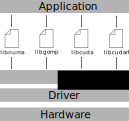
\includegraphics[width=0.5\textwidth]{figures/generated/app-abstraction.pdf}
    \caption[\todo{short}]{\todo{improve this figure}. The CUDA application interacts with the underlying hardware through libraries, the CUDA driver and the operating system.}
    \label{fig:app-abstraction}
\end{figure}

Through these layers of abstraction, the underlying communication capabilities are modified.
For example, PCIe interconnects transfer data with packets, but the CUDA API does not expose the ability to create custom packets to send to the GPU.
Furthermore, the performance of the hardware is modified.
For example, when CUDA unified memory is used, some of the link bandwidth may be consumed by control signals that help ensure data coherence.
Section~\ref{sec:results} shows how different uses of the CUDA API can achieve different performance on the same phyiscal hardware.


\section{Profiling Tooling}
\label{sec:profiling}

\subsection{CUDA Profiling Tools Interface}
\label{sec:cupti}

The CUDA Profiling Tools Interface~\cite{nvidia2017cupti} (CUPTI) ``provides...detailed information about how applications are using the GPU in a system.''
Users may inject code into the entry and exit point of every CUDA C Runtime and CUDA Driver API function call.
Additionally, users may configure and query hardware and software event counters to get insight into the operation of the GPU and CUDA stack.
The event counters include instruction count, instruction throughput, memory loads/stores, memory throughput, cache hits/misses, branches and custom profile triggers.
Chapter~\ref{ch:app-char} describes how \todo{hwcomm-apptracer} uses CUPTI to record memory allocations, kernel arguments, and timestamps to build a model of the application execution.

\subsection{\texttt{LD\_PRELOAD}}
\label{sec:ldpreload}

LD\_PRELOAD~\cite{kerrisk2017ld} is a mechanism by which the ld linker will load additional user-specific shared objects before any others.
If a function definition is present in a pre-loaded shared object, it will override the implementation present in later objects.
When combined with dlsym()~\cite{kerrisk2017dlysm}, it can be used to inject code into the entry of library calls in dynamically-linked binaries.
Chapter~\ref{ch:app-char} describes how \todo{hwcomm-apptracer} uses LD\_PRELOAD to record special information about cuBLAS and cuDNN calls.

\section{Linux Non-Uniform Memory Access}
\label{sec:numa}

Linux includes a system for exposing non-uniform memory access architectures (NUMA) to applications.
In NUMA systems, memory is devided into multiple \textit{nodes}\cite{numa2012}.
Processors and devices have the same access characteristics when accessing memory in a particular node.
Nodes have \textit{affinity} to processors and devices, indicating the processors and devices which can access that node with the best performance.
Applications can leverage the numactl\cite{wickman2015numactl} library to affect their own NUMA execution policy.
This policy controls on which CPUs processes may execute, and on which NUMA nodes memory is allocated.

\section{System Descriptions}
\label{ref:system-description}

Three high-performance heterogeneous systems are used in this work: an IBM S822LC for High Performance Computing ``Minsky''~\cite{caldeira2016s822lc}, an IBM AC922~\cite{caldeira2018ac922}, and an NVIDIA DGX-1~\cite{nvidia2016dgx1}.
All systems feature multiple GPUs and multiple socketed CPUs.
Their key differences are in CPU architecture (64-lit little-endian PowerPC for S822LC and AC922', x86-64 for DGX-1), number of GPUs (4 for the IBM machines, 8 for NVIDIA), and GPU connection topology (NVLink 1.0 for S822LC, NVLink 2.0 for AC922, and hybrid PCIe 3.0 / NVLink 1.0 for DGX-1).

\subsection{IBM S822LC for High Performance Computing ``Minsky''}
\label{sec:minsky-description}

\todo{where to discuss NUMA for each system?}

\begin{table}[]
    \centering
    \caption[Minsky hardware summary.]{
        Brief summary of Minsky hardware.
        }
    \label{tab:minsky}
    \begin{tabular}{|c|c|}
    \hline
    \textbf{} & \textbf{Specification}                              \\ \hline
    CPU           & \makecell{2x IBM Power8 \\ 20C / 80T \\ 4 GHz}  \\ \hline
    System Memory & 512 GB DDR4                                    \\ \hline
	GPU           & 4 NVIDIA P100                                   \\ \hline
	CPU/GPU Interconnect  & NVLink 1.0                                      \\ \hline
    \end{tabular}
\end{table}

The IBM S822LC ``Minsky'' machine features two POWER8 CPUs and four NVIDIA P100 GPUs\cite{caldeira2016s822lc}.
Each POWER8 CPU has 10 cores, with 8-way simultaneous multithreading, and is attached to 256GB of DDR4 memory. for a total of 160 threads and 512 GB of memory.
Each POWER8 CPU is part of a fully-connected triad of one POWER8 CPU and two P100 GPUs.
Each device in the triad is connected by a gang of two NVLink 1.0 lanes for a total bidirectional bandwidth of 80 GB/s.
The two triads are connected at the POWER8 CPUs by an IBM SMP X bus with 38.4 GB/s of bidirectional bandwidth.
Table~\ref{tab:minsky} summarizes the hardware configuration.

Figure \ref{fig:topo-minsky-simple} shows a simplified view\footnote{Figure \ref{fig:topo-minsky-actual} shows a detailed view.} of the topology discovered by \todo{hwcomm}.


\begin{figure}
    \centering
	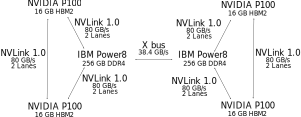
\includegraphics[width=0.8\textwidth]{figures/generated/minsky-hardware.pdf}
    \caption[Minsky Hardware]{\todo{Minsky}}
    \label{fig:topo-minsky-simple}
\end{figure}


\subsection{NVIDIA DGX-1}
\label{sec:dgx1-description}

\begin{table}[]
    \centering
    \caption[NVIDIA DGX-1 hardware summary.]{Summary of NVIDIA DGX-1 Hardware}
    \label{tab:dgx1}
    \begin{tabular}{|c|c|}
    \hline
    \textbf{} & \textbf{Specification}                                          \\ \hline
    CPU           & \makecell{2x Intel Xeon E5-2698 v4 \\ 40C / 80T \\ 2.2 GHz} \\ \hline
    System Memory & 512 GB DDR4                                                 \\ \hline
	GPU           & 4 NVIDIA P100                                               \\ \hline
	CPU/GPU Interconnect  & NVLink 1.0 / PCIe 3.0                                       \\ \hline
    \end{tabular}
\end{table}

The NVIDIA DGX-1 machine consists of two symmetric sections\cite{nvidia2017dgx1}.
Each section consists of one 20-core Intel Xeon E5-2698v4 CPUs with 2-way SMT.
Each CPU is connected to 256GB of DDR4 RAM.
Each section has 4 NVIDIA Tesla P100 GPUs coupled by single NVLinks.
The sections are connected by an Intel 9.6GT/s QPI bus between the CPUs providing 38.4 GB/s of bidirectional bandwidth, as well as NVLinks between corresponding GPUs.
The first CPU socket hosts the majority of the PCI devices on the system, including the network interfaces and the disks.
Table~\ref{tab:dgx1} summarizes the hardware configuration.
Figure \ref{fig:topo-dgx-simple} shows a simplified view\footnote{Figure ~\ref{fig:topo-dgx-actual} shows a detailed view.} of the topology discovered by \todo{hwcomm}.



\begin{figure}
    \centering
	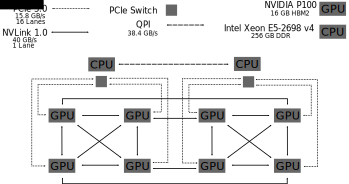
\includegraphics[width=0.8\textwidth]{figures/generated/dgx1-hardware.pdf}
    \caption[DGX-1 Hardware]{\todo{DGX-1}}
    \label{fig:topo-dgx-simple}
\end{figure}


\subsection{IBM AC922}
\label{sec:hal-description}

The IBM AC922 machine features two POWER9 CPUs and four NVIDIA V100 GPUs\cite{caldeira2018ac922}.
Each POWER9 CPU has 20 cores, with 4-way simultaneous multithreading, and is attached to 512GB of DDR4 memory. for a total of 160 threads and 1TB of memory.
Each POWER9 CPU is part of a fully-connected triad of one POWER9 CPU and two V100 GPUs.
Each device in the triad is connected by three bonded NVLink 2.0 lanes for bidirection bandwidth of 150 GB/s.
The two triads are connected at the POWER9 CPUs by an IBM SMP X bus with 64 GB/s bandwidth.
Table~\ref{tab:minsky} summarizes the hardware configuration.

\begin{table}[]
    \centering
    \caption[Power9 hardware summary.]{
        Brief summary of Power9 hardware.
        }
    \label{tab:hal}
    \begin{tabular}{|c|c|}
    \hline
    \textbf{} & \textbf{Specification}                              \\ \hline
    CPU           & \makecell{2x IBM Power9 \\ 40C 160T \\ 3.0 GHz  }  \\ \hline
    System Memory & 1TB DDR4                                   \\ \hline
	GPU           & 4 NVIDIA V100                                   \\ \hline
	CPU/GPU Interconnect  & NVLink 2.0                                      \\ \hline
    \end{tabular}
\end{table}

\begin{figure}
    \centering
	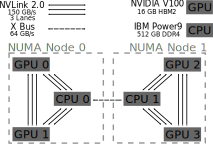
\includegraphics[width=0.8\textwidth]{figures/generated/hal-hardware.pdf}
    \caption[Power9 Hardware]{\todo{Power9}}
    \label{fig:topo-dgx-simple}
\end{figure}


\section{Parking Lot}

\subsection{Atomics}

\subsubsection{Atomic Operations prior to CC 6.0}

Beginning with CC 1.1 and continuing through CC 2.0, CUDA introduced an increasingly complete set of atomic operations, culminating in support for common 32-bit and 64-bit operations on integers and floating-point types in global and shared memory (\cite{nvidia2008cuda20} C.1)
All of these atomic operations were atomic with respect only to the executing GPU.

\subsubsection{Atomic Operations with CC 6.0+}

Compute Capability 6.0 brings two new kinds of atomics operations: system atomics (\texttt{atomic\*\_system}) and block atomics (\texttt{atomic\*\_block}) (\cite{nvidia2017cuda80}, B.12).
System atomics are atomic with respect to all CPUs and GPUs in the system.
Block atomics are atomic only with respect to other threads in the thread block.


\todo{cudaMemcpy and managed memory (J2.2.1)?}

\todo{Texture memory?}
%\subsubsection{Texture memory and CUDNN}
%\todo{3.2.11}

